\documentclass{article}
\usepackage{amsmath}
\usepackage{tikz}

\begin{document}

\begin{figure}[h]
    \centering
    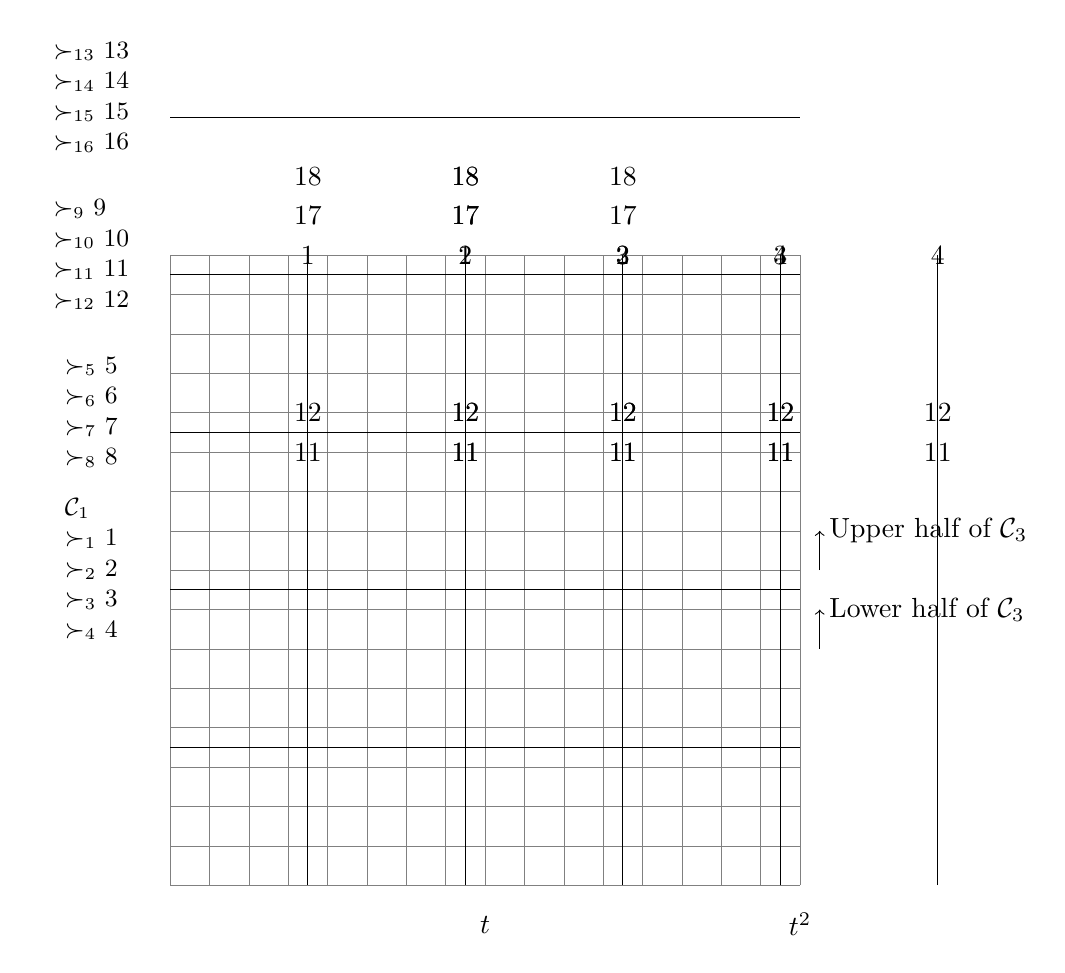
\begin{tikzpicture}[scale=0.5]
        % Draw the grid
        \draw[help lines] (0,0) grid (16,16);
        
        % Draw the horizontal bars
        \foreach \i in {1,2,...,4} {
            \draw (\i*4-0.5,0) -- (\i*4-0.5,16);
            \draw (\i*4+3.5,0) -- (\i*4+3.5,16);
        }
        
        % Draw the vertical bars
        \foreach \j in {1,2,...,4} {
            \draw (0,\j*4-0.5) -- (16,\j*4-0.5);
            \draw (0,\j*4+3.5) -- (16,\j*4+3.5);
        }
        
        % Mark the top-ranked alternatives
        \foreach \i in {1,2,...,4} {
            \node at (\i*4-0.5,16) {\i};
            \node at (\i*4+3.5,16) {\i};
        }
        
        % Mark the alternatives 11 and 12
        \foreach \i in {1,2,...,4} {
            \node at (\i*4-0.5,11) {11};
            \node at (\i*4-0.5,12) {12};
            \node at (\i*4+3.5,11) {11};
            \node at (\i*4+3.5,12) {12};
        }
        
        % Mark the alternatives 17 and 18
        \foreach \i in {1,2} {
            \node at (\i*4-0.5,17) {17};
            \node at (\i*4-0.5,18) {18};
            \node at (\i*4+3.5,17) {17};
            \node at (\i*4+3.5,18) {18};
        }
        
        % Draw the labels
        \node at (8,-1) {$t$};
        \node at (16,-1) {$t^2$};
        
        % Draw the legend
        \draw[->] (16.5,8) -- (16.5,9) node[right] {Upper half of $\mathcal{C}_3$};
        \draw[->] (16.5,6) -- (16.5,7) node[right] {Lower half of $\mathcal{C}_3$};
        
        % Caption
        \node at (-2,8) {\small
            \begin{tabular}{l}
                \textbf{$\mathcal{C}_1$} \\
                $\succ_1$ 1 \\
                $\succ_2$ 2 \\
                $\succ_3$ 3 \\
                $\succ_4$ 4 \\
            \end{tabular}
        };
        \node at (-2,12) {\small
            \begin{tabular}{l}
                $\succ_5$ 5 \\
                $\succ_6$ 6 \\
                $\succ_7$ 7 \\
                $\succ_8$ 8 \\
            \end{tabular}
        };
        \node at (-2,16) {\small
            \begin{tabular}{l}
                $\succ_9$ 9 \\
                $\succ_{10}$ 10 \\
                $\succ_{11}$ 11 \\
                $\succ_{12}$ 12 \\
            \end{tabular}
        };
        \node at (-2,20) {\small
            \begin{tabular}{l}
                $\succ_{13}$ 13 \\
                $\succ_{14}$ 14 \\
                $\succ_{15}$ 15 \\
                $\succ_{16}$ 16 \\
            \end{tabular}
        };
    \end{tikzpicture}
    
    \caption{An example of our lower bound construction in Theorem~\ref{thm:0/1_valued_1_query_lower_bound} where $m = 18$. Hence, we set $t=4$ and $n=t^2=16$ resulting in the profile $P$ shown above. In every agent's ranking (horizontal bars), the example mentions the top-ranked alternative. Additionally, we marked alternatives $11$ and $12$ in every ranking in order to showcase the symmetry of $P$. Alternatives $17$ and $18$ are shown for two agents of every cohort. Notice that these alternatives appear in the exact same positions of every agent's ranking.}
    \label{fig:lower_bound_example}
\end{figure}

\end{document}